\section{Resoconto attività di verifica}
In questa sezione vengono descritti e analizzati gli esiti delle attività di verifica svolte su tutti i documenti che vengono consegnati nelle varie revisioni di avanzamento del progetto.
	\subsection{Revisione dei Requisiti}
		\subsubsection{Verifica della documentazione}
		Per la verifica della documentazione viene utilizzata la tecnica del \glock{walkthrough}, che ha portato all'individuazione di errori frequenti, insieme alla tecnica di \glock{inspection}, che mira a cercare gli errori più frequenti, come descritto nel documento \dext{norme di progetto v. 1.0.0}\footnote{sezione §3.4.4.1}
		\subsubsection{Leggibilità documenti}
		Nel seguente grafico vengono riportati gli indici di \glock{Gulpease} dei documenti finora stesi.
		\begin{figure}[H]
			\centering
			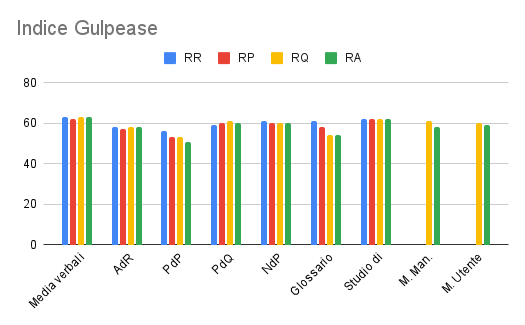
\includegraphics[width=0.7\linewidth]{res/images/IndiceGulpease.png}
			\caption*{\textbf{Figura 7}: Andamento dell'indice di Gulpease}
			\label{fig:Figura1}
		\end{figure}